%!TEX root = ../Thesis.tex
\chapter{Neural machine translation for automated feedback on children’s early-stage writing \\
\& \\ Supporting Children's Writing in Danish with Transformer Models}
In this Chapter I present our two papers related to WriteReader, the NLDL paper "Neural machine translation for automated feedback on children’s early-stage writing" and the pre-print "Supporting Children's Writing in Danish with Transformer Models". I choose to present them together here because the methodological contributions of the papers individually are perhaps not as large as the previous papers. Nevertheless, I include them because they are papers in which we showcase how probabilistic machine learning models can be used to improve downstream applications. Both of the projects stem from Michael's collaboration with the WriteReader startup whom were interested in using NLP models to automate the "translating" of children's writing to "conventional" writing in their ed-tech platform. For brief overview on sequence-to-sequence tasks which is the modelling task in these papers, please see Section \ref{sec:seqtoseq}. \\

\noindent In "Neural machine translation for
automated feedback on children’s
early-stage writing", we fine-tuned BART models for translating in English specifically. We presented a robust likelihood for handling the noisy data that WriteReader has collected (with parent consent) and showed how this improve the fine-tuning procedure. We then investigated how different methods for improving calibration in the Transformers performed and how one could use the likelihoods of predictive sequences to reject particularly bad samples which could be used for human-in-the-loop systems. In "Supporting Children's Writing in Danish with Transformer Models", we trained Transformer models completely from scratch\footnote{We do this due to the fact that there exist no pre-trained LLMs that have the same capacity as those in English.} for translating in Danish. In particular we looked at how different tokenisation strategies improved performance and calibration of the trained models both on in- and out-of distribution data. Finally, we showcased how the models can be used as parts of pipelines for performing automatic proficiency scoring \citep{AutomaticProficiencyWriting}.

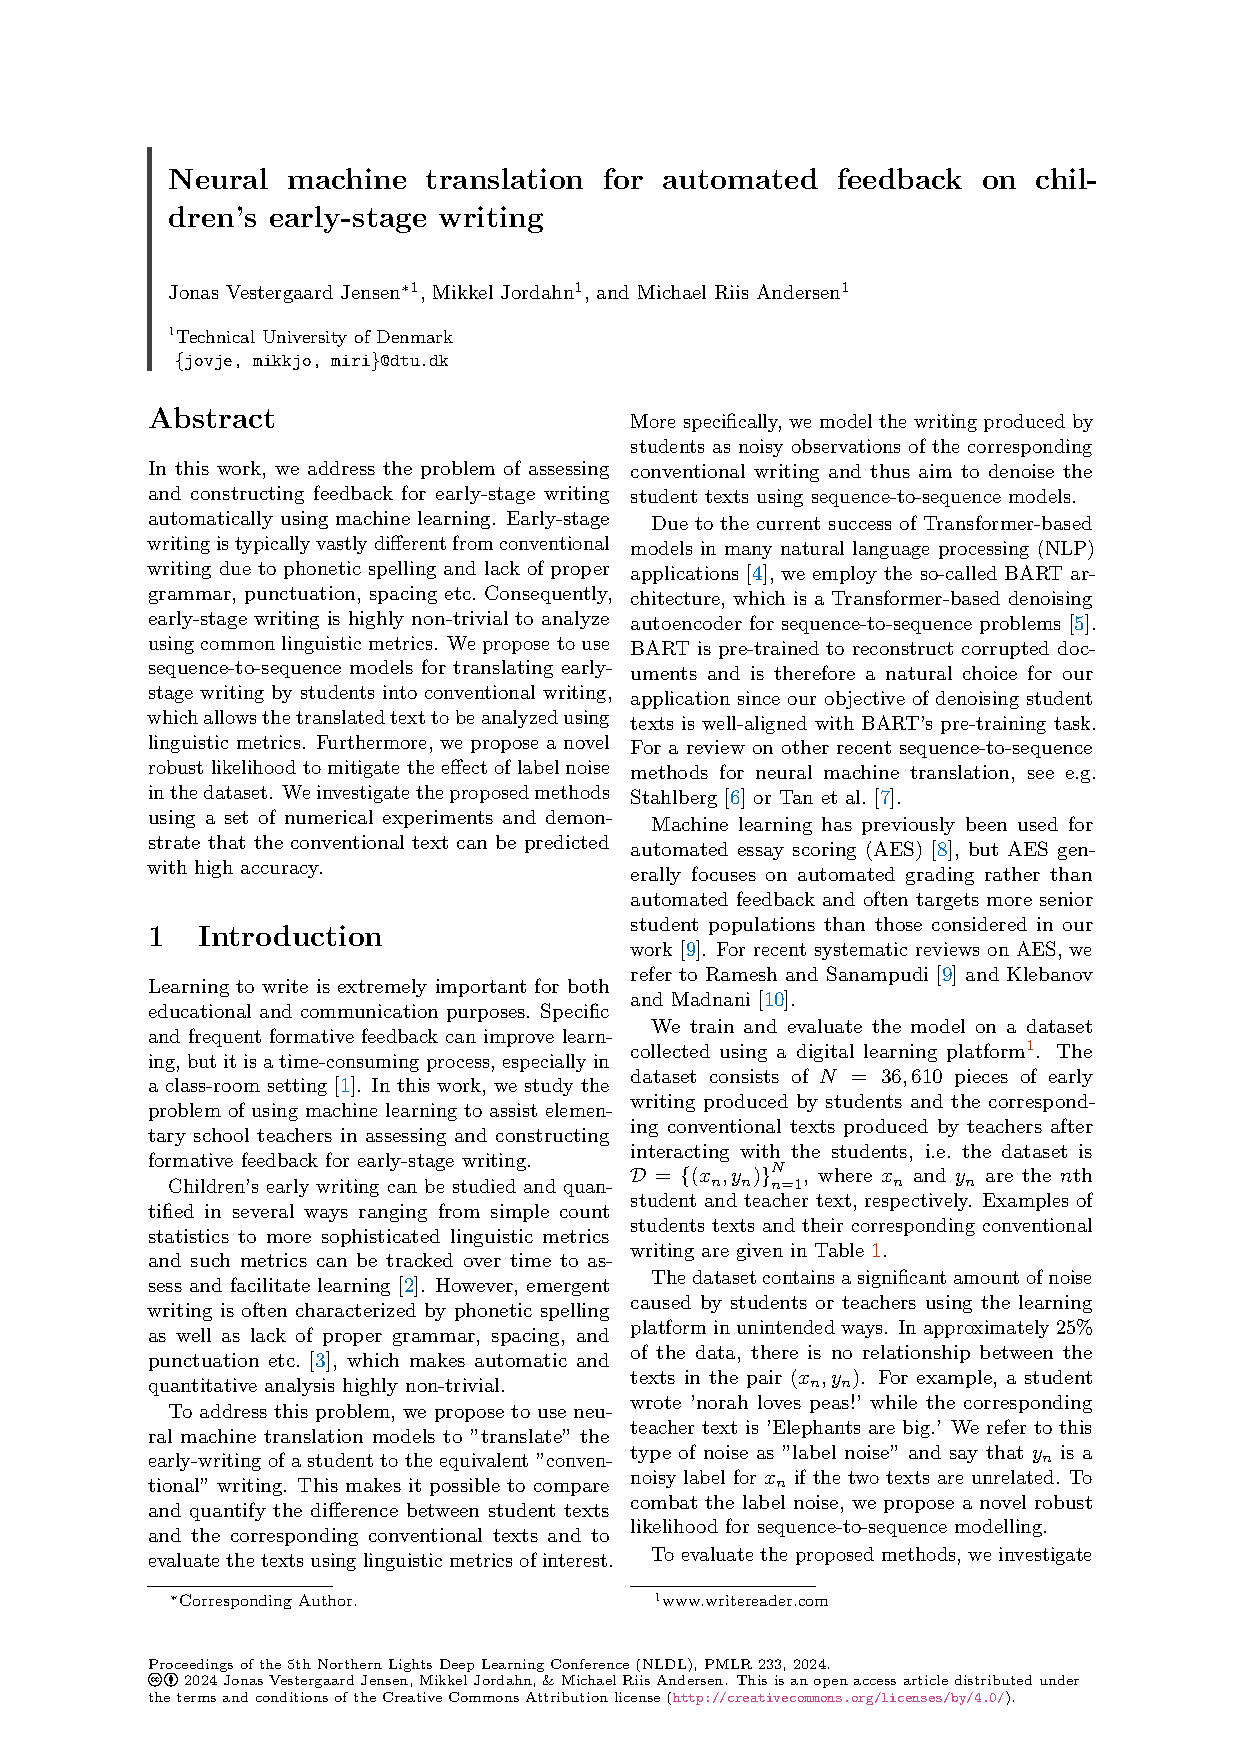
\includepdf[pages=-, offset=0mm 0mm, delta=0mm 0mm, scale=0.9, pagecommand={\thispagestyle{mystuff}{}{}{}}]{chapters/PaperEF_ATEL/Paper_NLDL.pdf}
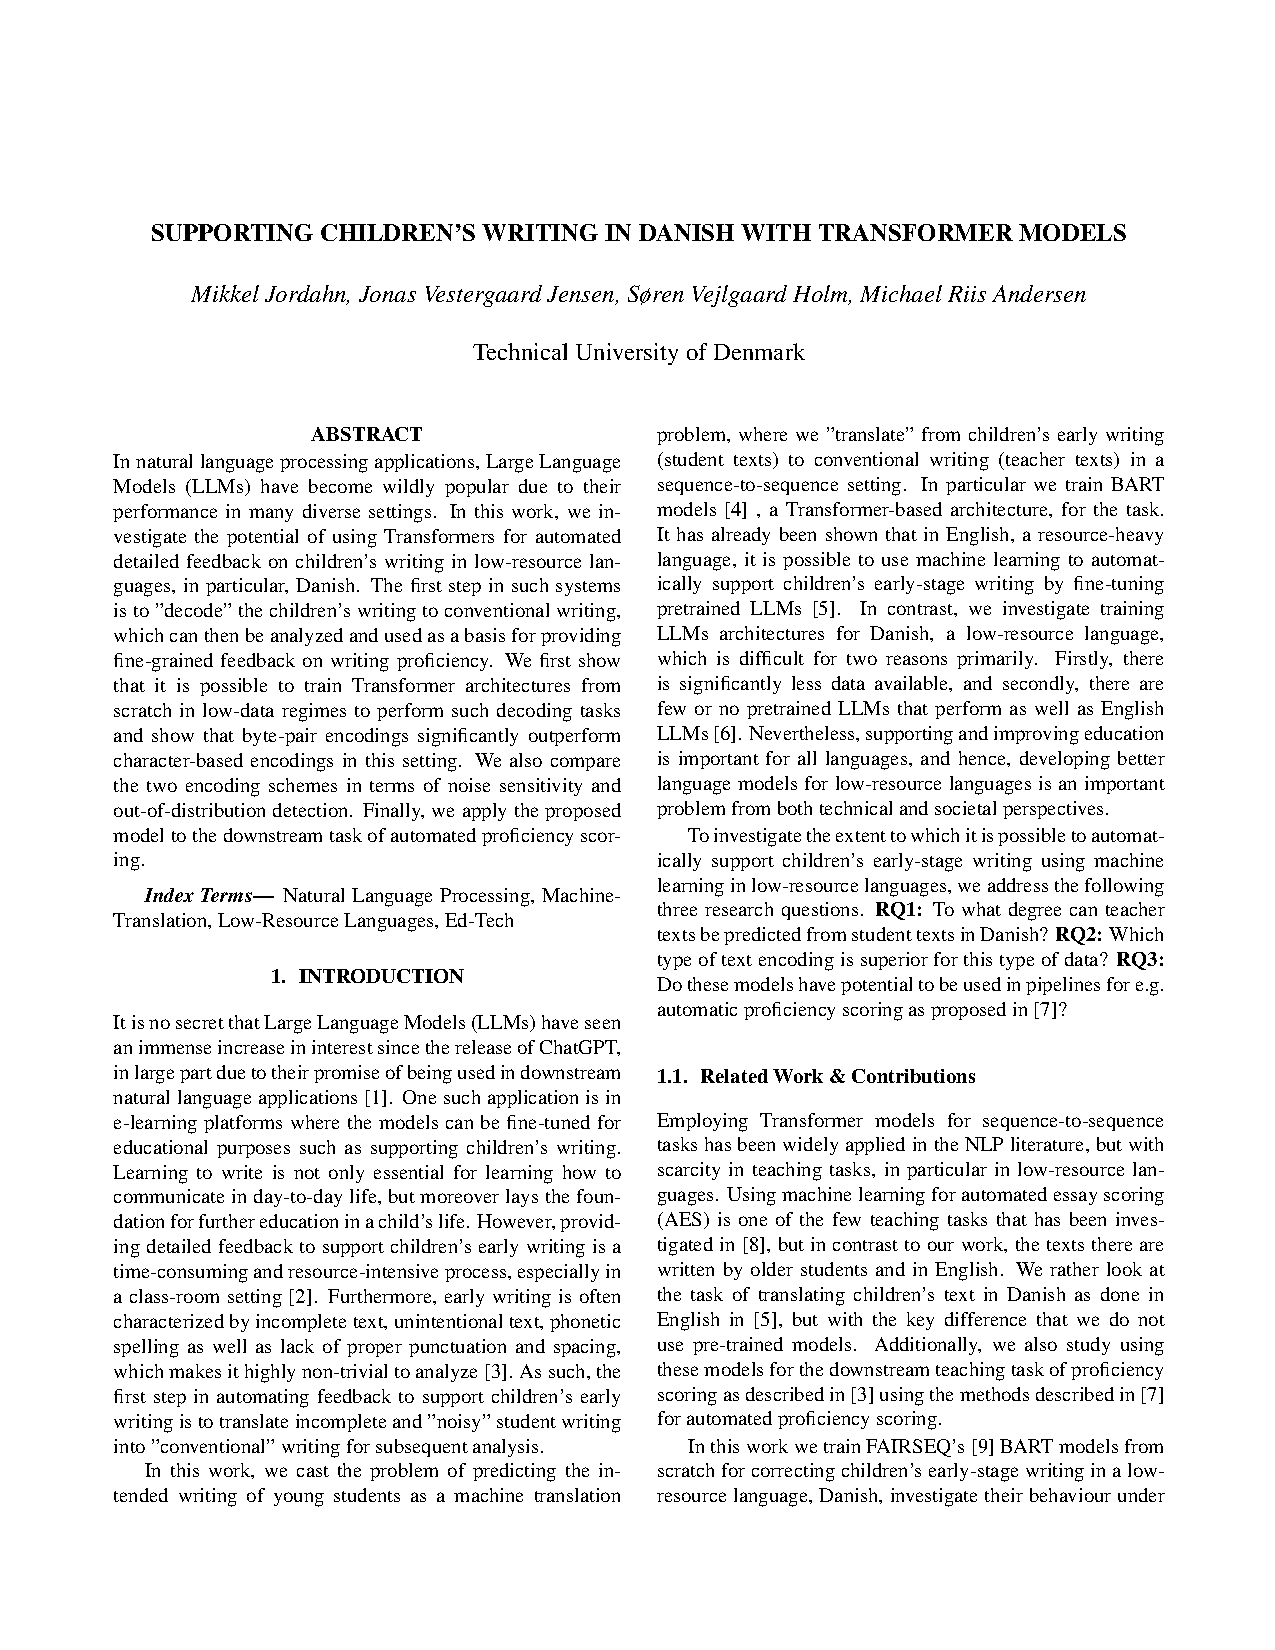
\includepdf[pages=-, offset=0mm 0mm, delta=0mm 0mm, scale=1.0, pagecommand={\thispagestyle{mystuff}{}{}{}}]{chapters/PaperEF_ATEL/Paper_MLSP}